\documentclass[screen,reqno]{aomart}
\usepackage{amsmath,amssymb,amsthm,mathtools}
\usepackage[utf8]{inputenc}
\usepackage{graphicx}
\usepackage[T1]{fontenc}
\usepackage{lmodern}
\usepackage{tikz-cd}
\usepackage{url}
\usepackage{xurl}
\hypersetup{pdftitle={The optimal log log q bound in the Polya-Vinogradov inequality},
pdfauthor={Deep Bhattacharjee; Ushashi Bhattacharya},
pdfsubject={Character-sum deductions using a precisely cited external zero-free theorem}}
\numberwithin{equation}{section}
\emergencystretch=3em
\raggedbottom
\makeatletter
\copyrightnote{}
\doinumber{}
\fancypagestyle{firstpage}{\fancyhf{}\renewcommand{\headrulewidth}{0pt}
\fancyhead[C]{\scriptsize Research draft, 24 October 2026}
\cfoot{\footnotesize\thepage}}
\makeatother
\newcommand{\releaseURL}{https://github.com/creelie/Breakthrough-problems-3}
\newcommand{\repoURL}{https://github.com/creelie/Breakthrough-problems-3}

\newtheorem{theorem}{Theorem}[section]
\newtheorem{lemma}[theorem]{Lemma}
\newtheorem{proposition}[theorem]{Proposition}
\newtheorem{corollary}[theorem]{Corollary}
\theoremstyle{definition}
\newtheorem{remark}[theorem]{Remark}

\renewcommand{\Re}{\operatorname{Re}}
\newcommand{\C}{\mathbb{C}}
\newcommand{\R}{\mathbb{R}}
\newcommand{\Z}{\mathbb{Z}}

\title[The optimal $\log\log q$ bound]{The optimal $\log\log q$ bound in the P\'olya--Vinogradov inequality}

\author[D. Bhattacharjee]{Deep Bhattacharjee}
\address{Formerly, Electro-Gravitational Space Propulsion Laboratory (EGSPL),
Bhubaneswar, Odisha 751030, India; Formerly, University of Calcutta, Senate House,
87/1 College Street, Kolkata 700073, West Bengal, India}
\email{itsdeep@live.com}
\email{d.bhattacharjee@erl-forschung.de}
\urladdr{https://orcid.org/0000-0003-0466-750X}
\thanks{Corresponding author: Deep Bhattacharjee. Earlier versions of this paper are the
Hexagon preprints \texttt{2610.00256v1} and \texttt{2610.00256v2},
\url{https://hexagonmath.org/2610.00256v2}.}

\author[U. Bhattacharya]{Ushashi Bhattacharya}
\address{Formerly, National Taiwan University, Taipei 106319, Taiwan}
\email{rai.bhattacharya.in@gmail.com}
\urladdr{https://orcid.org/0009-0002-2254-3914}

\subjclass[2020]{Primary 11L40; Secondary 11M06, 11M20, 11L07, 11N13, 11N36, 11R42}
\keywords{P\'olya--Vinogradov inequality, character sums, zero-free regions, Selberg sieve,
Euler--Kronecker constants}

\begin{document}

\begin{abstract}
Using OpenAI's uniform zero-free half-plane $\Re s>11/12$ for nonprincipal
Dirichlet $L$-functions, we derive the bound $C\sqrt q\log\log q$ for every
primitive Dirichlet character modulo $q\ge3$. The zero-free theorem is cited
as an external input. We give the subsequent contour, prime-sum, major-arc
and minor-arc arguments in detail and prove the required weak
Montgomery--Vaughan exponential-sum estimate using Selberg's sieve.
The same input yields $|L'/L(1,\chi)|\ll\log\log q$ and two-sided bounds
for cyclotomic Euler--Kronecker constants. Explicit parameters and a general
transfer argument show why any fixed uniform zero-free boundary below one
suffices. No independent proof of the external zero-free theorem is claimed.
\end{abstract}

\maketitle

\section{Introduction}

Let $\chi$ be a primitive Dirichlet character modulo $q\ge3$. The P\'olya--Vinogradov inequality
states that $\bigl|\sum_{n\le x}\chi(n)\bigr|\ll\sqrt q\log q$ uniformly in
$x$~\cite[Chapter~23]{Dav00}.\footnote{The proof expands $\chi$ in additive characters through the
Gauss sum $\tau(\bar\chi)$, whose modulus is $\sqrt q$ for primitive $\chi$, and bounds the
resulting geometric series trivially; Lemma~\ref{lem:polya} below is the same argument with the
harmonic sums kept.} Paley proved that the factor $\log q$ cannot be replaced by anything smaller
than $\log\log q$: for infinitely many primitive quadratic characters the maximum over $x$ exceeds
$c\sqrt q\log\log q$~\cite{Pal32}. Montgomery and Vaughan~\cite{MV77} proved the upper bound
$\sqrt q\log\log q$ under the generalised Riemann hypothesis. Without hypothesis, Granville and
Soundararajan lowered the exponent of $\log q$ for characters of fixed odd
order~\cite{GS07}.\footnote{For a primitive character of odd order $g$ they obtain
$\sqrt q(\log q)^{1-\delta_g/2+o(1)}$ with $\delta_g=1-\frac g\pi\sin\frac\pi g$, and under the
generalised Riemann hypothesis the same exponent of $\log\log q$.} We use the following precisely identified external theorem to obtain the bound of Montgomery and Vaughan.

\begin{theorem}[OpenAI, {\cite[Theorem 1.1]{OAI26short}}]
\label{thm:zerofree}
For every nonprincipal Dirichlet character $\xi$, one has
$L(s,\xi)\ne0$ whenever $\Re s>11/12$.
\end{theorem}

\begin{proof}[Source of the input]
This is the Dirichlet conclusion of Theorem~1.1 of~\cite{OAI26short}.
That paper's Section~3 deduces its theorem from Proposition~3.1, whose
proof is completed in Section~5.6. We invoke that result and do not
reproduce its article here. If the result is first stated for a primitive
character $\xi^*$, then an imprimitive $\xi$ has
\[
 L(s,\xi)=L(s,\xi^*)\prod_{p\mid q,\ p\nmid\operatorname{cond}(\xi^*)}
             (1-\xi^*(p)p^{-s}).
\]
The primitive inducing character is nonprincipal whenever $\xi$ is.
Each finite factor is nonzero for $\Re s>0$, since its second term has
modulus less than one. Thus the same boundary holds at imprimitive levels.
\end{proof}

\begin{theorem}[Using the cited zero-free input]\label{thm:pv}
There is an absolute constant $C$ such that for every primitive character
$\chi$ modulo $q\ge3$ and every $x\ge1$,
\[
  \Bigl|\sum_{n\le x}\chi(n)\Bigr|\le C\sqrt q\log\log q.
\]
\end{theorem}

By Paley's theorem the order of this upper bound is optimal. The
deductions in this article begin after Theorem~\ref{thm:zerofree}; the
zero-free theorem is explicitly attributed to its source. An independent
proof of that theorem by the present authors is not claimed. The stronger
formal development cited in~\cite{OAI26} is a separate verification route
for the external input. Appendix~\ref{app:parameters} gives the explicit
constants at the boundary $11/12$, and Appendix~\ref{app:uniformtransfer}
proves the transfer for every fixed boundary strictly smaller than one.

Montgomery and Vaughan use the Riemann hypothesis in one place: on the major arcs, for prime sums
of the characters $\chi\psi$ twisted by additive characters, where $\psi$ runs over the characters
of a small modulus $r$. A power saving in these sums is enough there, and
Theorem~\ref{thm:zerofree} provides one (Corollary~\ref{cor:prime}). On the minor arcs they use
their unconditional bound for exponential sums with multiplicative coefficients. A weaker form of
it suffices, and we prove that form in Section~\ref{sec:mv} with Selberg's sieve as the only
arithmetic input. Figure~\ref{fig:flow} shows how the parts fit together.

\begin{figure}[ht]
\centering
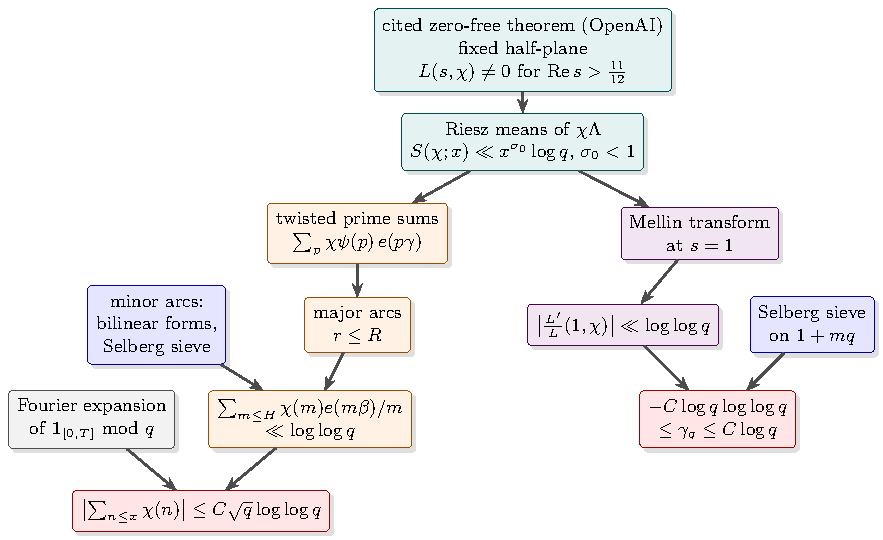
\includegraphics[width=\textwidth]{figures/fig_flow.pdf}
\caption{The structure of the proofs. The left branch proves Theorem~\ref{thm:pv}: the
Fourier expansion of a character sum reduces it to the sums
$\sum_{m\le H}\chi(m)e(m\beta)/m$, which are bounded on the major arcs by the half-plane and on
the minor arcs by bilinear forms and the sieve. The right branch proves
Theorem~\ref{thm:ek}.}
\label{fig:flow}
\end{figure}

The same half-plane controls the logarithmic derivative of $L(s,\chi)$ at $s=1$. For a number
field $K$ write $\zeta_K(s)=c_{-1}(s-1)^{-1}+c_0+O(s-1)$ near $s=1$; the Euler--Kronecker
constant of $K$ is $\gamma_K=c_0/c_{-1}$. Let $\gamma_q$ be the Euler--Kronecker constant of
$\mathbb Q(\zeta_q)$. For a prime $q$ the factorisation $\zeta_{\mathbb Q(\zeta_q)}(s)
=\zeta(s)\prod_{\chi\ne\chi_0}L(s,\chi)$, the product over the nonprincipal characters modulo
$q$~\cite[Theorem~4.3]{Was97},\footnote{All nonprincipal characters modulo a prime are
primitive, so no Euler factors have to be removed: the conductor of each nonprincipal $\chi$ is
$q$ itself, and $L(s,\chi)$ is the $L$-function of the corresponding primitive character.} gives
\begin{equation}\label{eq:gammaq}
  \gamma_q=\gamma+\sum_{\chi\ne\chi_0}\frac{L'}{L}(1,\chi),
\end{equation}
where $\gamma$ is Euler's constant.

\begin{theorem}\label{thm:ek}
Using Theorem~\ref{thm:zerofree}, there is an absolute constant $C$ with the following properties.
\begin{enumerate}
\item[(i)] For every nonprincipal character $\chi$ modulo $q$,
\[
  \Bigl|\frac{L'}{L}(1,\chi)\Bigr|\le C\log\log q.
\]
\item[(ii)] For every prime $q\ge3$,
$-C\log q\log\log q\le\gamma_q\le C\log q$.
\end{enumerate}
\end{theorem}

Under the generalised Riemann hypothesis the bound~(i) is classical, Ihara proved
$\gamma_q\le(2+o(1))\log q$ and Badzyan proved a lower bound of the order
of~(ii)~\cite{Iha06,Bad10}. Ford, Luca and Moree proved the two bounds of~(ii) without hypothesis
for a set of primes $q$ of density one~\cite{FLM14,Mor18}.\footnote{The difficulty for an
individual prime $q$ lies in the prime powers $n\equiv1\pmod q$, which enter $\gamma_q$ with the
weight $(q-1)\Lambda(n)/n$. Below $q^{25}$ we bound them for each prime $q$ separately by
Lemma~\ref{lem:progression}; beyond $q^{25}$ the zero-free half-plane makes their contribution
bounded.} For all primes the best unconditional bound we know is
$|\gamma_q|\ll_\varepsilon q^\varepsilon$, due to Ihara, Murty and Shimura~\cite{IMS09}. The
upper bound in~(ii) needs only Chebyshev's bound. The lower bound needs an upper bound for the
prime powers $n\le q^{25}$ with $n\equiv1\pmod q$, which we obtain from Selberg's sieve applied
in dyadic blocks (Lemma~\ref{lem:progression}).

The arguments of Theorems~\ref{thm:pv} and~\ref{thm:ek} work, with other constants, whenever $L(s,\chi)\ne0$ on $\Re s>\theta$ for all nonprincipal $\chi$
and some fixed $\theta<1$.
The paper is organised as follows. Section~\ref{sec:prelim} collects Chebyshev's bounds and
Selberg's sieve. Section~\ref{sec:riesz} bounds Riesz means of $\chi\Lambda$ by a contour shift.
Section~\ref{sec:mv} proves the bound for exponential sums with multiplicative coefficients,
Section~\ref{sec:pv} proves Theorem~\ref{thm:pv} and Section~\ref{sec:ek} proves
Theorem~\ref{thm:ek}.

\section{Preliminaries}\label{sec:prelim}

Throughout, $p$ and $\ell$ denote primes, $\Lambda$ is the von Mangoldt function,
$\theta(x)=\sum_{p\le x}\log p$, $\psi(x)=\sum_{n\le x}\Lambda(n)$, $e(x)=e^{2\pi ix}$, and
$\|x\|$ is the distance from $x$ to the nearest integer. We write $\omega(n)$ for the number of
prime factors of $n$, $\tau_3(n)$ for the number of ordered factorisations $n=abc$, and $P(n)$
for the largest prime factor of $n\ge2$, with $P(1)=1$.

\begin{lemma}\label{lem:chebyshev}
For $x\ge1$ and integers $N\ge2$,
\begin{enumerate}
\item[(i)] $\theta(x)\le x\log4$;
\item[(ii)] $\psi(x)-\theta(x)\le2\sqrt x\log x$ and $\psi(x)\le4x$;
\item[(iii)] $\sum_{p\le N}\frac{\log p}p\le\log N+\log4$;
\item[(iv)] $\sum_{p\le N}\frac1p\le\log\log N+10$.
\end{enumerate}
\end{lemma}

\begin{proof}
(i) It suffices to treat integers $m\ge1$, and we use induction on $m$. The cases $m=1,2$ are
clear, and for even $m>2$ we have $\theta(m)=\theta(m-1)$. Let $m=2n+1$. The primes in
$(n+1,2n+1]$ divide $\binom{2n+1}n$, and $2\binom{2n+1}n\le2^{2n+1}$ because $\binom{2n+1}n$ and
$\binom{2n+1}{n+1}$ are equal terms of the binomial expansion of $(1+1)^{2n+1}$. Hence
$\theta(2n+1)\le\theta(n+1)+n\log4\le(2n+1)\log4$.

(ii) We have $\psi(x)-\theta(x)=\sum_{k\ge2}\theta(x^{1/k})$, where only $k\le\log x/\log2$
contribute. Each term is at most $\sqrt x\log4$ by~(i), so the sum is at most
$(\log x/\log2)\sqrt x\log4=2\sqrt x\log x$. Since $\log x\le\sqrt x$, $\psi(x)\le(\log4+2)x\le4x$.

(iii) By Legendre's formula and~(i),
\[
  N\log N\ge\log N!\ge\sum_{p\le N}\Bigl\lfloor\frac Np\Bigr\rfloor\log p
  \ge N\sum_{p\le N}\frac{\log p}p-N\log4.
\]

(iv) Let $A(u)=\sum_{p\le u}\log p/p$. Partial summation and~(iii) give
\[
  \sum_{p\le N}\frac1p=\frac{A(N)}{\log N}+\int_2^N\frac{A(u)}{u\log^2u}\,du
  \le1+\frac{\log4}{\log2}+\int_2^N\Bigl(\frac1{u\log u}+\frac{\log4}{u\log^2u}\Bigr)du,
\]
and the integral is at most $\log\log N-\log\log2+2$.
\end{proof}

We use Selberg's upper bound sieve in the following form; for the method
see~\cite[Chapter~3]{HR74}, and we give the proof of the form we need.\footnote{The weights
$\lambda_d$ are those of Selberg's quadratic form, and the only feature used later is the bound
$|\lambda_d|\le1$, which makes the remainder term at most a sum of $3^{\omega(d)}|R_d|$ over
$d\le y$.}

\begin{lemma}\label{lem:selberg}
Let $a_1,\dots,a_X$ be integers, $P$ a squarefree integer, $\nu$ a multiplicative function with
$0<\nu(p)<1$ for $p\mid P$, and $y\ge1$. For $d\mid P$ put
$R_d=\#\{n\le X:d\mid a_n\}-\nu(d)X$, and for $l\mid P$ put
$g(l)=\prod_{p\mid l}\nu(p)/(1-\nu(p))$. Then
\[
  \#\{n\le X:(a_n,P)=1\}\le\frac XS+\sum_{\substack{d\mid P\\d\le y}}3^{\omega(d)}|R_d|,
  \qquad S=\sum_{\substack{l\mid P\\l\le\sqrt y}}g(l).
\]
\end{lemma}

\begin{proof}
Let $D$ be the set of divisors $d$ of $P$ with $d\le\sqrt y$, and let $(\lambda_d)_{d\in D}$ be
real numbers with $\lambda_1=1$. If $(a_n,P)=1$ then $\sum_{d\in D,\,d\mid a_n}\lambda_d=1$, and
otherwise this sum is real, so
\begin{align*}
  \#\{n:(a_n,P)=1\}&\le\sum_{n\le X}\Bigl(\sum_{\substack{d\in D\\d\mid a_n}}\lambda_d\Bigr)^2\\
  &=X\sum_{d_1,d_2\in D}\lambda_{d_1}\lambda_{d_2}\nu([d_1,d_2])
  +\sum_{d_1,d_2\in D}\lambda_{d_1}\lambda_{d_2}R_{[d_1,d_2]}.
\end{align*}
Write $Q$ for the double sum in the first term. Since $\nu$ is multiplicative and $d_1,d_2$ are
squarefree, $\nu([d_1,d_2])=\nu(d_1)\nu(d_2)/\nu((d_1,d_2))$. Let $h$ be the multiplicative
function on the divisors of $P$ with $h(p)=1/\nu(p)-1=1/g(p)$; then $1/\nu(m)=\sum_{l\mid m}h(l)$
for $m\mid P$, and
\[
  Q=\sum_{l\mid P}h(l)\Bigl(\sum_{\substack{d\in D\\l\mid d}}\lambda_d\nu(d)\Bigr)^2
  =\sum_{l\in D}\frac{y_l^2}{g(l)},\qquad y_l=\sum_{\substack{d\in D\\l\mid d}}\lambda_d\nu(d).
\]
M\"obius inversion gives $\lambda_d\nu(d)=\sum_{l\in D,\,d\mid l}\mu(l/d)y_l$, so the condition
$\lambda_1=1$ reads $\sum_{l\in D}\mu(l)y_l=1$. By Cauchy's inequality
\[
  1\le\Bigl(\sum_{l\in D}\frac{y_l^2}{g(l)}\Bigr)\Bigl(\sum_{l\in D}g(l)\Bigr)=QS,
\]
with equality for $y_l=\mu(l)g(l)/S$. We make this choice, so that $Q=1/S$. Then, writing
$l=de$,
\[
  \lambda_d=\frac{1}{\nu(d)S}\sum_{\substack{l\in D\\d\mid l}}\mu(l/d)\mu(l)g(l)
  =\frac{\mu(d)g(d)}{\nu(d)S}\sum_{\substack{e\in D,\ (e,d)=1\\de\le\sqrt y}}g(e).
\]
Since $g(d)/\nu(d)=\prod_{p\mid d}(1-\nu(p))^{-1}=\prod_{p\mid d}(1+g(p))=\sum_{f\mid d}g(f)$, we
get $|\lambda_d|\le S^{-1}\sum_{f\mid d}\sum_eg(fe)$, and the products $fe$ are distinct elements
of $D$; hence $|\lambda_d|\le1$. Finally $[d_1,d_2]\le d_1d_2\le y$, and every $d\mid P$ is the
least common multiple of at most $3^{\omega(d)}$ pairs $(d_1,d_2)$, so the second term is at most
$\sum_{d\mid P,\,d\le y}3^{\omega(d)}|R_d|$.
\end{proof}

\section{Riesz means of prime sums}\label{sec:riesz}

For an arithmetic function $a$ and $x\ge1$ put
\[
  S(a;x)=\sum_{n\le x}a(n)\Bigl(1-\frac nx\Bigr),\qquad
  S(\chi;x)=S(\chi\Lambda;x)=\sum_{n\le x}\chi(n)\Lambda(n)\Bigl(1-\frac nx\Bigr).
\]
The weight $1-n/x$ makes the Mellin kernel absolutely integrable, which keeps the contour shift
below free of truncation errors. The aim of this section is Proposition~\ref{prop:riesz}.

\begin{lemma}\label{lem:mellin}
Let $a\colon\mathbb N\to\C$ satisfy $\sum_n|a(n)|n^{-\sigma}<\infty$ for $\sigma>1$, and let
$F(s)=\sum_na(n)n^{-s}$ for $\Re s>1$.
\begin{enumerate}
\item[(i)] For $\Re s>1$, $\displaystyle\int_1^\infty S(a;x)\,x^{-s-1}\,dx=\frac{F(s)}{s(s+1)}$.
\item[(ii)] For $x>0$, $\displaystyle S(a;x)=\frac1{2\pi}\int_{-\infty}^{\infty}
F(2+it)\,\frac{x^{2+it}}{(2+it)(3+it)}\,dt$.
\end{enumerate}
In other words the following square commutes, and~(ii) inverts its right column on the line
$\Re s=2$:
\[
\begin{tikzcd}[column sep=6em,row sep=3em]
a \arrow[r,"\text{Riesz mean}"] \arrow[d,"\text{Dirichlet series}"'] &
S(a;\cdot) \arrow[d,"\text{Mellin transform}"] \\
F \arrow[r,"\times\,\frac1{s(s+1)}"'] & \dfrac{F(s)}{s(s+1)}
\end{tikzcd}
\]
\end{lemma}

\begin{proof}
(i) For $n\ge1$, $\int_n^\infty(1-n/x)x^{-s-1}dx=n^{-s}/s-n^{-s}/(s+1)=n^{-s}/(s(s+1))$. Since
$\sum_n|a(n)|\int_n^\infty x^{-\sigma-1}dx=\sigma^{-1}\sum_n|a(n)|n^{-\sigma}<\infty$, the sum
and the integral may be exchanged.

(ii) For $y>0$ let $k(y)=\frac1{2\pi i}\int_{(2)}y^s\,\frac{ds}{s(s+1)}$. If $y\ge1$, moving the
line of integration to $\Re s=-U$, with $U>2$, picks up the residues $1$ at $s=0$ and
$-1/y$ at $s=-1$. For each fixed $U$, the horizontal integrals tend to zero as their
height tends to infinity: their lengths are fixed and the denominator is of order
the square of that height. On the new vertical line,
\[
 \int_{-\infty}^{\infty}\frac{|y^{-U+it}|}{|(-U+it)(1-U+it)|}\,dt
 \le y^{-U}\int_{-\infty}^{\infty}\frac{dt}{(U-1)^2+t^2}
 =\frac{\pi y^{-U}}{U-1}.
\]
This tends to zero for $y\ge1$, including $y=1$, so $k(y)=1-1/y$ there.
For $y<1$, shifting instead to $\Re s=U$ crosses no pole and leaves an integral
bounded by $\pi y^U/U$, which tends to zero. As
$|s(s+1)|^{-1}$ is integrable on $\Re s=2$ and $\sum_n|a(n)|n^{-2}<\infty$, summation and
integration may be exchanged, and the right side equals $\sum_na(n)k(x/n)=S(a;x)$.
\end{proof}

\begin{lemma}\label{lem:size}
Let $\chi$ be nonprincipal modulo $q$. For $\Re s=\sigma>0$, $|L(s,\chi)|\le q|s|/\sigma$.
\end{lemma}

\begin{proof}
Put $A(t)=\sum_{n\le t}\chi(n)$; then $|A(t)|\le q$, and partial summation gives
$L(s,\chi)=s\int_1^\infty A(t)t^{-s-1}\,dt$ for $\sigma>0$. Hence
$|L(s,\chi)|\le q|s|\int_1^\infty t^{-\sigma-1}dt=q|s|/\sigma$.
\end{proof}

\begin{lemma}\label{lem:euler}
Let $A_0=\frac32\sum_\ell\ell^{-3/2}$. For every Dirichlet character $\chi$ the series
$E(s)=-\sum_\ell\log(1-\chi(\ell)\ell^{-s})$ is holomorphic on $\Re s>1$, $e^{E(s)}=L(s,\chi)$
there, and $|E(s)|\le A_0$ for $\Re s\ge3/2$.
\end{lemma}

\begin{proof}
For $\Re s\ge1$ we have $|\chi(\ell)\ell^{-s}|\le1/2$, and $|\log(1-w)|\le\sum_k|w|^k/k
\le\frac32|w|$ for $|w|\le1/2$: indeed, the terms with $k\ge2$ have total at most
$|w|^2/(2(1-|w|))\le |w|/2$. The series therefore converges locally uniformly on $\Re s>1$
and is bounded by $A_0$ on $\Re s\ge3/2$, and the Euler product gives $e^E=L$.
\end{proof}

\begin{lemma}[Borel--Carath\'eodory]\label{lem:bc}
Let $h$ be holomorphic on a neighbourhood of the disc $|z-c|\le R$ and let $0<r<R$. Then
\[
  \max_{|z-c|\le r}|h(z)-h(c)|\le\frac{2r}{R-r}\max_{|w-c|=R}\Re\bigl(h(w)-h(c)\bigr).
\]
\end{lemma}

\begin{proof}
Put $g(z)=h(c+z)-h(c)$ and $A=\max_{|w|=R}\Re g(w)$. The mean of $\Re g$ over the circle
$|w|=R$ is $\Re g(0)=0$, so $A\ge0$. If $A=0$, then $\Re g$ vanishes on the circle, hence on the
disc, and $g$ is an imaginary constant equal to $g(0)=0$. Let $A>0$. By the maximum principle
$\Re g\le A$ on $|z|\le R$, so $|2A-g|\ge A$ there and $\phi=g/(2A-g)$ is holomorphic. Since
$|g|^2-|2A-g|^2=4A(\Re g-A)\le0$, we have $|\phi|\le1$, and $\phi(0)=0$. Schwarz's lemma gives
$|\phi(z)|\le|z|/R$, and from $g=2A\phi/(1+\phi)$ we get $|g(z)|\le2A|z|/(R-|z|)$.
\end{proof}

\begin{lemma}\label{lem:logderiv}
Let $0<\delta<1/1000$, $1/2\le a\le1$, and let $\chi$ be nonprincipal modulo $q$ with
$L(s,\chi)\ne0$ for $\Re s>a+2\delta$. Put $K_1=(1+2A_0)/(2\delta^2)$. For
$a+8\delta\le\sigma\le2$ and $t\in\R$,
\[
  \Bigl|\frac{L'}{L}(\sigma+it,\chi)\Bigr|\le K_1\log\bigl(2q(3+|t|)^2\bigr).
\]
\end{lemma}

\begin{proof}
Let $c=2+it$, $R=2-a-3\delta$, $r=2-a-6\delta$ and $\Lambda_0=\log(2q(3+|t|)^2)\ge\log18>1$.
On the disc $|z-c|<2-a-2\delta$ we have $\Re z>a+2\delta$, so $L(z,\chi)$ has no zero there
and has a holomorphic logarithm $h$. On $|z-c|<1/2$ both $h$ and the function $E$ of
Lemma~\ref{lem:euler} are logarithms of $L$, so they differ by a constant in $2\pi i\Z$; we
choose $h=E$ there. Then $|h(c)|\le A_0$.

If $|z-c|\le R$, then $\Re z\ge a+3\delta\ge1/2$ and $|z|\le|c|+3/2\le4+|t|$, so
Lemma~\ref{lem:size} gives $\Re h(z)=\log|L(z,\chi)|\le\log(2q(4+|t|))\le\Lambda_0$.
Lemma~\ref{lem:bc} gives, for $|z-c|\le r$,
\[
  |h(z)-h(c)|\le\frac{2r}{R-r}\bigl(\Lambda_0+A_0\bigr)\le\frac{\Lambda_0+A_0}{\delta},
\]
as $r\le3/2$ and $R-r=3\delta$. Hence $|h(z)|\le A_0+(\Lambda_0+A_0)/\delta\le(1+2A_0)\Lambda_0/\delta$
on $|z-c|\le r$. For $w=\sigma+it$ with $a+8\delta\le\sigma\le2$ we have $|w-c|=2-\sigma\le r-2\delta$,
so the circle $|z-w|=2\delta$ lies in $|z-c|\le r$, and Cauchy's estimate gives
$|L'/L(w,\chi)|=|h'(w)|\le(1+2A_0)\Lambda_0/(2\delta^2)$.
\end{proof}

\begin{lemma}\label{lem:elementary}
For $q\ge1$, $t\in\R$ and $s=\sigma+it$ with $\sigma\ge1/2$,
\[
  \log\bigl(2q(3+|t|)^2\bigr)\le10\log(q+2)(1+|t|)^{1/2},\qquad |s(s+1)|\ge\tfrac18(1+|t|)^2.
\]
\end{lemma}

\begin{proof}
We have $\log(2q)\le2\log(q+2)$, and $\log y\le2y^{1/2}$ with $3+|t|\le4(1+|t|)$ gives
$\log(3+|t|)\le4(1+|t|)^{1/2}$; the first bound follows from $\log(q+2)\ge1$. For the second,
$|s|\ge\max(\sigma,|t|)\ge(1+|t|)/4$ and $|s+1|\ge\max(\sigma+1,|t|)\ge(1+|t|)/2$.
\end{proof}

\begin{proposition}\label{prop:riesz}
Let $0<\delta<1/1000$. There is $K=K(\delta)$ such that the following holds. Let $1/2\le a\le1$
and let $\chi$ be nonprincipal modulo $q$ with $L(s,\chi)\ne0$ for $\Re s>a+2\delta$. Then for
$x\ge1$,
\[
  |S(\chi;x)|\le K\,x^{a+8\delta}\log(q+2).
\]
\end{proposition}

\begin{proof}
Put $\sigma_0=a+8\delta$ and
\[
  \Phi(s)=-\frac{L'}{L}(s,\chi)\,\frac{x^s}{s(s+1)}.
\]
For $\Re s>1$, $-L'/L(s,\chi)=\sum_n\chi(n)\Lambda(n)n^{-s}$, so Lemma~\ref{lem:mellin}(ii) gives
$S(\chi;x)=\frac1{2\pi}\int\Phi(2+it)\,dt$. The function $\Phi$ is holomorphic on
$\sigma_0\le\Re s\le2$, and by Lemmas~\ref{lem:logderiv} and~\ref{lem:elementary},
\[
  |\Phi(\sigma+it)|\le80K_1\log(q+2)\,x^{\sigma}(1+|t|)^{-3/2}\qquad(\sigma_0\le\sigma\le2).
\]
This tends to $0$ as $|t|\to\infty$ uniformly in $\sigma$, so Cauchy's theorem on the rectangles
$[\sigma_0,2]\times[-T,T]$, $T\to\infty$, moves the integral to $\Re s=\sigma_0$
(Figure~\ref{fig:splane}). Since $\int_\R(1+|t|)^{-3/2}dt=4$, we get
$|S(\chi;x)|\le\frac{160K_1}{\pi}x^{\sigma_0}\log(q+2)$.
\end{proof}

\begin{figure}[ht]
\centering
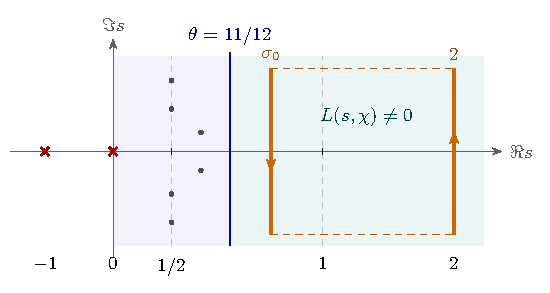
\includegraphics[width=\textwidth]{figures/fig_splane.pdf}
\caption{The contour shift in the proof of Proposition~\ref{prop:riesz}. The indicated nontrivial zeros of
$L(s,\chi)$ lie in $0\le\Re s\le11/12$ (dots), the kernel $x^s/(s(s+1))$ has poles at
$0$ and $-1$ (crosses), and the line of integration moves from $\Re s=2$ to
$\Re s=\sigma_0$ inside the zero-free half-plane. Horizontal spacing is schematic.}
\label{fig:splane}
\end{figure}

From now on fix $\delta=1/2000$ and $a=11/12-1/1000$, so that $a+2\delta=11/12$ and
\[
  \sigma_0=a+8\delta=\frac{11}{12}+\frac3{1000},
\]
and let $K$ be the constant of Proposition~\ref{prop:riesz} for this $\delta$. By
Theorem~\ref{thm:zerofree}, Proposition~\ref{prop:riesz} applies to every nonprincipal character.

\begin{corollary}\label{cor:prime}
There is an absolute constant $C_3$ such that for every nonprincipal character $\xi$ modulo $k$:
\begin{enumerate}
\item[(i)] $|S(\xi;x)|\le Kx^{\sigma_0}\log(k+2)$ for $x\ge1$;
\item[(ii)] $\bigl|\sum_{p\le x}\xi(p)\log p\bigr|\le C_3x^{49/50}\log(k+2)$ for $x\ge1$;
\item[(iii)] for integers $2\le A\le B$ and $\gamma\in\R$,
\begin{equation}\label{eq:twistedprime}
  \Bigl|\sum_{A<p\le B}\xi(p)e(p\gamma)\Bigr|\le
  2C_3\,\frac{B^{49/50}\log(k+2)(2+2\pi|\gamma|B)}{\log A}.
\end{equation}
\end{enumerate}
\end{corollary}

\begin{proof}
(i) is Proposition~\ref{prop:riesz}. For (ii) put $T(y)=yS(\xi;y)$, that is,
$T(y)=\sum_{n\le y}\xi(n)\Lambda(n)(y-n)$, and let $0<h\le x$. Then
\[
  T(x+h)-T(x)=h\sum_{n\le x}\xi(n)\Lambda(n)+\sum_{x<n\le x+h}\xi(n)\Lambda(n)(x+h-n),
\]
and the last sum has at most $h+1$ terms, each of modulus at most $h\log(2x)$. With
$|T(y)|\le Ky^{1+\sigma_0}\log(k+2)$ this gives
\[
  \Bigl|\sum_{n\le x}\xi(n)\Lambda(n)\Bigr|\le\frac{2K(2x)^{1+\sigma_0}\log(k+2)}h+(h+1)\log(2x).
\]
Take $h=x^{47/50}$. Since $1+\sigma_0-47/50<49/50$ and $\log(2x)\le1+100x^{1/100}$, the right side
is at most $(8K+202)x^{49/50}\log(k+2)$. The prime powers contribute at most
$\psi(x)-\theta(x)\le2\sqrt x\log x\le200x^{49/50}$ by Lemma~\ref{lem:chebyshev}(ii), and~(ii)
follows with $C_3=8K+402$.

(iii) Let $\Pi(u)=\sum_{p\le u}\xi(p)\log p$ and $f(u)=e(u\gamma)/\log u$. Partial summation gives
\[
  \sum_{A<p\le B}\xi(p)e(p\gamma)=f(B)\Pi(B)-f(A)\Pi(A)-\int_A^B\Pi(u)f'(u)\,du,
\]
and $|f'(u)|\le2\pi|\gamma|/\log A+1/(u\log^2u)$ for $u\ge A$. By~(ii) the right side is at most
$C_3B^{49/50}\log(k+2)\bigl(3+2\pi|\gamma|B\bigr)/\log A$, which gives~\eqref{eq:twistedprime}.
\end{proof}

\section{Exponential sums with multiplicative coefficients}\label{sec:mv}

For $M>0$ put $w_M(\theta)=M$ if $\|\theta\|<1/M$ and $w_M(\theta)=1/\|\theta\|$ otherwise;
then $0\le w_M(\theta)\le M$ and $w_M(-\theta)=w_M(\theta)$.

\begin{theorem}\label{thm:mv}
There is an absolute constant $C_1$ with the following property. Let $f$ be completely
multiplicative with $|f(n)|\le1$, let $\alpha\in\R$, and let $a,r$ be coprime integers with
$r\ge1$, $|\alpha-a/r|\le r^{-2}$ and $2\le R\le r\le N/R$. Then
\[
  \Bigl|\sum_{n\le N}f(n)e(n\alpha)\Bigr|\le C_1\Bigl(\frac N{\log N}
  +\frac{N(\log N)^2}{R^{1/4}}\Bigr).
\]
\end{theorem}

Montgomery and Vaughan~\cite[Corollary~1]{MV77} proved this for multiplicative $f$ with
$N(\log R)^{3/2}R^{-1/2}$ in place of $N(\log N)^2R^{-1/4}$. The proof below follows their
approach, a bilinear decomposition together with the spacing of the multiples of $\alpha$ and an
upper bound for prime pairs, with cruder estimates, which suffice for Theorem~\ref{thm:pv}.

\begin{lemma}\label{lem:spacing}
Let $a,r$ be coprime with $r\ge2$ and $|\alpha-a/r|\le r^{-2}$, and let $H\ge0$ be an integer.
\begin{enumerate}
\item[(i)] $\|k\alpha\|\ge1/(2r)$ for every integer $k$ with $0<|k|\le r/2$.
\item[(ii)] $\#\{1\le h\le H:\|h\alpha\|<t\}\le(4H/r+1)(4rt+1)$ for every $t\ge0$.
\item[(iii)] For $M>0$ and every integer $K\ge0$ with $M\le2^K$,
\begin{align*}
  \sum_{h\le H}w_M(h\alpha)&\le\Bigl(\frac{4H}r+1\Bigr)(3M+4r+8rK),\\
  \sum_{h\le H}w_M(h\alpha)^2&\le\Bigl(\frac{4H}r+1\Bigr)(20rM+3M^2).
\end{align*}
\end{enumerate}
\end{lemma}

\begin{proof}
(i) Let $z$ be the integer nearest to $k\alpha$. Since $0<|k|<r$ and $(a,r)=1$, $r\nmid ka$, so
$|ka/r-z|\ge1/r$ and $\|k\alpha\|\ge1/r-|k|\,|\alpha-a/r|\ge1/(2r)$.

(ii) Let $L=\lfloor r/2\rfloor$, so $L\ge r/4$. For $k$ in a block of $L$ consecutive integers let
$y_k=k\alpha-z_k$ with $z_k$ the integer nearest to $k\alpha$. For $k\ne k'$ in the block,
$0<|k-k'|<L\le r/2$ and $y_k-y_{k'}\equiv(k-k')\alpha\pmod1$, so $|y_k-y_{k'}|\ge1/(2r)$ by~(i).
Points of $(-t,t)$ at mutual distances at least $1/(2r)$ number at most $4rt+1$, and $[1,H]$ is
covered by at most $H/L+1\le4H/r+1$ blocks.

(iii) If $\|\theta\|\ge1/M$, let $k\ge1$ be least with $\|\theta\|<2^k/M$; then $k\le K$ because
$\|\theta\|\le1/2<2^K/M$, and $\|\theta\|\ge2^{k-1}/M$, so $w_M(\theta)\le2^{1-k}M$. Hence
\[
  w_M(\theta)^j\le M^j\,[\|\theta\|<1/M]+\sum_{k=1}^K(2^{1-k}M)^j\,[\|\theta\|<2^k/M]\qquad(j=1,2).
\]
Summing over $h\le H$ with~(ii), the first sum is at most
$(4H/r+1)\bigl(4r+M+\sum_{k\le K}(8r+2^{1-k}M)\bigr)$ and the second at most
$(4H/r+1)\bigl(4rM+M^2+\sum_{k\ge1}(16rM2^{-k}+4M^24^{-k})\bigr)$.
\end{proof}

\begin{lemma}\label{lem:bilinear}
Let $\theta,\alpha\in\R$, $U>0$, and let $A,B,N$ be nonnegative integers with $B\le A+U$.
\begin{enumerate}
\item[(i)] $\bigl|\sum_{A<x\le B}e(x\theta)\bigr|\le w_U(\theta)$.
\item[(ii)] For a finite set $V$ of positive integers and $b:V\to\C$,
\[
  \sum_{A<u\le B}\Bigl|\sum_{\substack{v\in V\\uv\le N}}b(v)e(uv\alpha)\Bigr|^2\le
  \sum_{v,v'\in V}|b(v)|\,|b(v')|\,w_U\bigl((v-v')\alpha\bigr).
\]
\item[(iii)] For $M>0$ and an integer $H\ge0$,
$\sum_{1\le m,m'\le H}w_M((m-m')\alpha)\le H\bigl(M+2\sum_{h\le H}w_M(h\alpha)\bigr)$.
\end{enumerate}
\end{lemma}

\begin{proof}
(i) If $\|\theta\|<1/U$, the sum has at most $U$ terms of modulus $1$. Otherwise
$\theta\notin\Z$, the sum has modulus at most $|e((B-A)\theta)-1|/|e(\theta)-1|$, and
$|e(\theta)-1|=2|\sin\pi\theta|\ge4\|\theta\|$, so the modulus is at most $1/(2\|\theta\|)$.
(ii) Expanding the square gives $\sum_{v,v'}b(v)\overline{b(v')}\sum_ue(u(v-v')\alpha)$, where
$u$ runs over the integers of $(A,\min(B,N/v,N/v')]$, an interval of length at most $U$; apply~(i).
(iii) For fixed $m$, the term $m'=m$ is $w_M(0)=M$, and each $h=|m-m'|\in[1,H]$ arises from at
most two $m'$.
\end{proof}

\begin{lemma}\label{lem:reduction}
Let $C_5=1+4\zeta(3/2)$. For every completely multiplicative $f$ with $|f(n)|\le1$, every
$\alpha\in\R$ and every integer $N\ge1$, the sum $S=\sum_{n\le N}f(n)e(n\alpha)$ satisfies
\[
  \Bigl|S\log N-\sum_{p\le N}\log p\,f(p)\sum_{m\le N/p}f(m)e(pm\alpha)\Bigr|\le C_5N.
\]
\end{lemma}

\begin{proof}
Write $S\log N=S_1+S_2$ with $S_1=\sum_{n\le N}f(n)e(n\alpha)\log n$ and
$S_2=\sum_{n\le N}f(n)e(n\alpha)\log(N/n)$. Then $|S_2|\le N\log N-\log N!\le N$, since
$N^N/N!\le e^N$. In $S_1$ write $\log n=\sum_{d\mid n}\Lambda(d)$ and $n=dm$; complete
multiplicativity gives $\sum_{d\le N}\Lambda(d)f(d)\sum_{m\le N/d}f(m)e(dm\alpha)$. The terms with
$d$ prime form the sum in the statement, and the others have modulus at most
$N\sum_p\sum_{k\ge2}\log p/p^k\le2N\sum_p\log p/p^2\le4\zeta(3/2)N$, since $\log p\le2\sqrt p$.
\end{proof}

Let $G(h)=\prod_{p\mid h}p/(p-1)$.

\begin{lemma}\label{lem:pairs}
\begin{enumerate}
\item[(i)] For every integer $X\ge2$ and every even $h\ge2$,
\[
  \#\{0\le n<X:n\text{ and }n+h\text{ prime}\}\le\frac{400\,G(h)^2X}{(\log X)^2}+3X^{3/5}.
\]
\item[(ii)] $\sum_{h\le X}G(h)^4\le e^{30}X$ for every $X\ge1$.
\end{enumerate}
\end{lemma}

\begin{proof}
(i) Apply Lemma~\ref{lem:selberg} to $a_n=n(n+h)$, $0\le n<X$, with $y=X^{1/5}$,
$z=\lfloor y\rfloor$, $P$ the product of the primes $p\le z$ with $p\nmid h$, and
$\nu(d)=2^{\omega(d)}/d$. Every $p\mid P$ is odd, so $\nu(p)=2/p<1$. For $d\mid P$ the residues $n$
with $d\mid n(n+h)$ form $2^{\omega(d)}$ classes modulo $d$ (namely $n\equiv0$ or $-h\pmod p$ for
each $p\mid d$, distinct as $p\nmid h$), and each class contains between $X/d-1$ and $X/d+1$ of
the integers $0\le n<X$; hence $|R_d|\le2^{\omega(d)}$. Since the prime factors of $d$ are at
least $3$, $3^{\omega(d)}|R_d|\le6^{\omega(d)}\le d^2\le y^2$, and the error term is at most
$y^3=X^{3/5}$.

Let $\mathcal M$ be the set of $m\le\sqrt y$ whose prime factors divide $P$. Since
$\nu(p)/(1-\nu(p))=\sum_{k\ge1}\nu(p)^k$ and $\nu(m)=2^{\Omega(m)}/m$ for these $m$, $g(l)$ is the
sum of $2^{\Omega(m)}/m$ over the $m$ whose set of prime factors is that of $l$. An $m\in\mathcal M$
is counted in $g(l)$ for $l$ the product of its prime factors, and $l\le m\le\sqrt y$. Hence,
with $\tau(m)\le2^{\Omega(m)}$ the number of divisors of $m$,
\[
  S\ge\sum_{m\in\mathcal M}\frac{2^{\Omega(m)}}m\ge\sum_{m\in\mathcal M}\frac{\tau(m)}m.
\]
Let $T=\lfloor y^{1/4}\rfloor$ and let $B$ be
the set of $b\le T$ that are prime to $h$; these $b$ are odd. For $b,b'\in B$ the product $bb'$
lies in $\mathcal M$, and a given $m$ is a product $bb'$ in at most $\tau(m)$ ways, so
$S\ge\bigl(\sum_{b\in B}1/b\bigr)^2$. If $E$ is a set of primes and $p\notin E$, every $b\le T$
prime to $E$ is uniquely $p^kb'$ with $b'$ prime to $E\cup\{p\}$, so the sum of $1/b$ over the
$b\le T$ prime to $E$ is at most $p/(p-1)$ times the same sum for $E\cup\{p\}$. Adding the prime
factors of $h$ one at a time gives
\[
  \sum_{b\in B}\frac1b\ge\frac1{G(h)}\sum_{b\le T}\frac1b\ge\frac{\log(T+1)}{G(h)}.
\]
As $T+1>y^{1/4}=X^{1/20}$, we get $S\ge(\log X)^2/(400G(h)^2)$, that is,
$X/S\le400G(h)^2X/(\log X)^2$. Finally, if $n<X$ and both $n$ and $n+h$ are prime, then
$n\le z$ or $(n(n+h),P)=1$, so the count is at most $z+1+X/S+y^3\le400G(h)^2X/(\log X)^2+3X^{3/5}$.

(ii) For $t=p-1\ge1$, $(t+1)^5\le(t+31)t^4$, that is, $(p/(p-1))^4\le1+30/p$. Hence
$G(h)^4\le\sum_d30^{\omega(d)}/d$ over the squarefree $d\mid h$, and
\begin{align*}
  \sum_{h\le X}G(h)^4&\le\sum_{d\le X}\mu(d)^2\frac{30^{\omega(d)}}d\cdot\frac Xd
  \le X\prod_p\Bigl(1+\frac{30}{p^2}\Bigr)\\
  &\le X\exp\Bigl(30\sum_{n\ge2}\frac1{n^2}\Bigr)\le e^{30}X.\qedhere
\end{align*}
\end{proof}

\begin{proof}[Proof of Theorem~\ref{thm:mv}]
Let $S$ be the sum in the theorem, $L=\log N$ and $\ell=\lfloor\log_2N\rfloor$. Since
$N\ge rR\ge4$, we have $L\ge1$. If $\ell<64$, then $L<64\log2<45$ and $|S|\le N\le45N/L$. Let now
$\ell\ge64$, and put $I=\lfloor\log_2\ell\rfloor+1$ and $J=\ell+1-4I$. Then $16^I>\ell^4$, $1\le J\le\ell\le2L$,
$I\le\ell\le2L$, $2^I\le2\ell$, $N<2^{\ell+1}=2^J16^I$ and
$J^22^J\le(\ell+1)^22^{\ell+1}\ell^{-4}\le2N$. By Lemma~\ref{lem:reduction},
$|S|L\le C_5N+|T_1|+|T_2|$, where $T_1$ and $T_2$ are the parts of
$\sum_p\log p\,f(p)\sum_{m\le N/p}f(m)e(pm\alpha)$ with $p\le2^J$ and with $p>2^J$.

\emph{The small primes.} Let $0\le j<J$, $U=2^j$, $H=\lfloor N/U\rfloor$, and for $U<x\le2U$ let
$B(x)=\sum_{m\le H,\,xm\le N}f(m)e(xm\alpha)$; the inner sum for a prime $p\in(U,2U]$ is $B(p)$.
By Cauchy's inequality, Lemma~\ref{lem:bilinear}(ii), (iii) and Lemma~\ref{lem:spacing}(iii) with
$M=U$, $K=j$,
\[
  \sum_{U<p\le2U}\log p\,|B(p)|\le\bigl(U\log^2(2U)\bigr)^{1/2}Q_j^{1/2},
\]
where $Q_j=H\bigl(U+2(4H/r+1)(3U+4r+8rj)\bigr)$.
Since $HU\le N$, $UQ_j\le7NU+(8+16j)Nr+24N^2/r+(32+64j)N^2/U$, and $\log(2U)\le j+1$. Summing over
$j<J$ with $j+1\le J$, $\sum_{j<J}2^{j/2}\le3\cdot2^{J/2}$,
$\sqrt{(32+64j)2^{-j}}\le8(j+1)(3/4)^j$ and $\sum_{j\ge0}(j+1)^2(3/4)^j=112$,
\[
  |T_1|\le3\sqrt7J\sqrt{N2^J}+J^2N\sqrt{24/r}+896N+J^2\sqrt{24JNr}.
\]
Now $J^22^J\le2N$ gives $3\sqrt7J\sqrt{N2^J}\le12N$; $r\ge R\ge\sqrt R$ gives
$\sqrt{24/r}\le5R^{-1/4}$; and $r\sqrt R\le rR\le N$ gives $\sqrt{24JNr}\le5JNR^{-1/4}$. With
$J\le2L$ and $L\ge1$, $|T_1|\le908N+60L^3NR^{-1/4}$.

\emph{The large primes.} For $p>2^J$ we have $N/p<16^I$, so the $m$ in $T_2$ lie in
$(0,16^I-1]$, the union of the blocks $(16^i-1,16^{i+1}-1]$ with $0\le i<I$. Fix $i$, let
$A=16^i-1$, $U=15\cdot16^i$ and $X=\lfloor N/16^i\rfloor$, and assume $X\ge1$, the block being
empty otherwise. Only the primes $p\in(2^J,X]$ contribute, since $p\ge X+1$ and $m\ge16^i$ give
$pm>N$. Let $V$ be the set of these primes, which are odd, and
$B(m)=\sum_{p\in V,\,pm\le N}\log p\,f(p)e(pm\alpha)$. The block is
$\sum_{A<m\le A+U}f(m)B(m)$, and by Cauchy's inequality, Lemma~\ref{lem:bilinear}(ii) and
$\log p\le\lambda=\log(X+1)$, its square is at most $U\lambda^2W$, where
\[
  W=\sum_{p,p'\in V}w_U((p-p')\alpha)=|V|U+2\sum_{h=1}^Xw_U(h\alpha)\,\#\{p\in V:p+h\in V\}.
\]
The count vanishes for odd $h$, and for even $h$ Lemma~\ref{lem:pairs}(i), applied to $X+1$,
bounds it by $400G(h)^2(X+1)\lambda^{-2}+3(X+1)^{3/5}$. By Cauchy's inequality,
Lemma~\ref{lem:pairs}(ii) and Lemma~\ref{lem:spacing}(iii),
$\sum_{h\le X}G(h)^2w_U(h\alpha)\le e^{15}\sqrt XQ^{1/2}$ with $Q=(4X/r+1)(20rU+3U^2)$, and
$\sum_{h\le X}w_U(h\alpha)\le XU$. Hence $U\lambda^2W\le A_1+800e^{15}Z+A_3$, where
\[
  A_1=U^2\lambda^2X,\qquad Z=U(X+1)\sqrt XQ^{1/2},\qquad A_3=6U^2\lambda^2(X+1)^{3/5}X.
\]
Let $\kappa=\log(N+1)\ge\lambda$ and $T_i=4^i\kappa\,(N(2N)^{3/5})^{1/2}$. Since
$U^2X=225\cdot16^i(16^iX)\le225\cdot16^iN$ and $X+1\le2N$, we get $A_1\le225T_i^2$ and
$A_3\le1350T_i^2\le37^2T_i^2$. With $w=UX\le15N$, $X\le N/16^i$ and $R\le r\le N/R$,
\begin{align*}
  Z^2\le4U^2X^3Q&=320w^3X+\frac{48w^4}r+80rw^3+12Uw^3\\
  &\le\frac{320\cdot15^3N^4}{16^i}+\frac{48\cdot15^4N^4}R+\frac{80\cdot15^3N^4}R\\
  &\qquad+180\cdot15^3\cdot16^iN^3,
\end{align*}
and every coefficient is at most $40^4$, so $Z^{1/2}\le40(N2^{-i}+2NR^{-1/4}+2^iN^{3/4})$. The
block is therefore at most
\begin{align*}
  &15T_i+40\sqrt{800e^{15}}\bigl(N2^{-i}+2NR^{-1/4}+2^iN^{3/4}\bigr)+37T_i\\
  &\qquad\le K_b\bigl(N2^{-i}+NR^{-1/4}+2^iN^{3/4}+T_i\bigr),
\end{align*}
with $K_b=80\sqrt{800e^{15}}+52$. Summing over $i<I$,
\[
  |T_2|\le K_b\bigl(2N+INR^{-1/4}+2^IN^{3/4}+4^I\kappa(N(2N)^{3/5})^{1/2}\bigr).
\]
Here $I\le2L^3$; $2^I\le4L\le16N^{1/4}$; $4^I\le16L^2$ and $\kappa\le2L$; and
$\log x\le15x^{1/15}$ gives $L^3(N(2N)^{3/5})^{1/2}\le2\cdot15^3N$. Hence
$|T_2|\le K_b(216018N+2L^3NR^{-1/4})$.

Altogether $|S|L\le(C_5+908+216018K_b)N+(60+2K_b)L^3NR^{-1/4}$, and dividing by $L$ gives the
theorem with $C_1=45+C_5+908+216018K_b+60+2K_b$.
\end{proof}

\section{Proof of Theorem~\ref{thm:pv}}\label{sec:pv}

In this section $\chi$ is a primitive character modulo $q\ge3$.

\begin{lemma}\label{lem:polya}
Let $B\ge0$ be such that $\bigl|\sum_{m\le H}\bar\chi(m)e(m\beta)/m\bigr|\le B$ for every integer
$H\le q/2$ and every $\beta\in\R$. Then $\bigl|\sum_{n\le x}\chi(n)\bigr|\le\sqrt q\,(B+6)$ for
every $x\ge0$.
\end{lemma}

\begin{proof}
We may take $x=T$ to be an integer. Let $\tau=\sum_{a\bmod q}\bar\chi(a)e(a/q)$. Since
$\bar\chi$ is primitive, $\sum_a\bar\chi(a)e(an/q)=\chi(n)\tau$ for every $n$, and summing the
squares of the moduli of these identities over $n\bmod q$ gives $q\varphi(q)=|\tau|^2\varphi(q)$,
so $|\tau|=\sqrt q$. Summing over $1\le n\le T$,
\[
  \tau\sum_{n\le T}\chi(n)=\sum_{0<|a|\le q/2}\bar\chi(a)\,
  \frac{e(aT/q)-1}{1-e(-a/q)},
\]
where $a$ runs over the integers with $-q/2<a\le q/2$, $a\ne0$. For $0<|\theta|\le1/2$ put
$r(\theta)=(1-e(-\theta))^{-1}-(2\pi i\theta)^{-1}$; then $|1-e(-\theta)|=2|\sin\pi\theta|\ge4|\theta|$.
If $2\pi|\theta|\le1$, then $|e(-\theta)-1+2\pi i\theta|\le(2\pi\theta)^2$ and
$|r(\theta)|\le(2\pi\theta)^2/(4|\theta|\cdot2\pi|\theta|)<3$; otherwise
$|r(\theta)|\le1/(4|\theta|)+1/(2\pi|\theta|)<3$. The terms with $r(a/q)$ contribute at most
$6q$. Writing $a=\pm m$ with $1\le m\le q/2$, the remaining terms are $q/(2\pi i)$ times a
combination, with coefficients of modulus at most $1$, of four sums
$\sum_{m\le H}\bar\chi(m)e(m\beta)/m$ with $H\le q/2$, so they contribute at most $2qB/\pi$.
Dividing by $|\tau|$ gives the claim.
\end{proof}

\begin{lemma}\label{lem:smooth}
For $Y\ge2$ and $H\ge1$,
\[
  \sum_{\substack{n\le H\\P(n)\le Y}}\frac1n\le e^{11}\log Y.
\]
\end{lemma}

\begin{proof}
The sum is at most $\prod_{p\le Y}(1-1/p)^{-1}\le\exp\bigl(\sum_{p\le Y}\frac1{p-1}\bigr)$, and
$\sum_p\bigl(\frac1{p-1}-\frac1p\bigr)\le1$; apply Lemma~\ref{lem:chebyshev}(iv).
\end{proof}

\begin{lemma}\label{lem:major}
There is an absolute constant $C_2$ such that for $0<r<q$, $b\in\Z$, $\beta\in\R$, integers
$Y\ge\max(2,r)$ and $t\ge1$,
\[
  \Bigl|\sum_{\substack{n\le t\\P(n)>Y}}\chi(n)e\Bigl(n\Bigl(\frac br+\beta\Bigr)\Bigr)\Bigr|
  \le C_2\,\frac{r\log(qr+2)\,(2+2\pi|\beta|t)\,t}{Y^{1/50}\log Y}.
\]
\end{lemma}

\begin{proof}
Every $n\le t$ with $P(n)>Y$ is uniquely $n=pm$ with $p=P(n)$ prime, $Y<p\le t/m$ and
$P(m)\le p$, and then $m\le t/Y$. For such $p$ we have $p>r$, so $p\nmid r$, and on the units
modulo $r$ the function $u\mapsto e(umb/r)$ equals $\sum_\psi c_\psi\psi(u)$, the sum over the
characters $\psi$ modulo $r$, with $|c_\psi|\le1$.

The character $\chi\psi$ modulo $qr$ is nonprincipal. Otherwise $\chi(n)=\bar\psi(n)$ for every
$n$ prime to $qr$. Let $d=(q,r)$ and let $n$ be prime to $q$ with $n\equiv1\pmod d$. By the
Chinese remainder theorem there is $n'$ prime to $qr$ with $n'\equiv n\pmod q$ and
$n'\equiv1\pmod r$, and then $\chi(n)=\chi(n')=\bar\psi(n')=1$. So $\chi$ is trivial on the
units congruent to $1$ modulo $d$, and is induced by a character modulo $d\le r<q$, which
contradicts primitivity.

Applying~\eqref{eq:twistedprime} to $\xi=\chi\psi$ with $\gamma=m\beta$,
$A=\max(Y,P(m)-1)$ and $B=\lfloor t/m\rfloor$ (the inner sum is empty if $A\ge B$) gives
\[
  \Bigl|\sum_{\substack{n\le t\\P(n)>Y}}\chi(n)e\Bigl(n\Bigl(\frac br+\beta\Bigr)\Bigr)\Bigr|
  \le2C_3r\,\frac{\log(qr+2)(2+2\pi|\beta|t)}{\log Y}\sum_{m\le t/Y}\Bigl(\frac tm\Bigr)^{49/50},
\]
and $\sum_{m\le M}m^{-49/50}\le50M^{1/50}$. Hence $C_2=100C_3$ will do.
\end{proof}

\begin{proposition}\label{prop:hsum}
There is an absolute constant $C_4$ such that if $\log q\ge200$, then
$\bigl|\sum_{m\le H}\chi(m)e(m\beta)/m\bigr|\le C_4\log\log q$ for every integer $H\le q$ and
every $\beta\in\R$.
\end{proposition}

\begin{proof}
Let $L=\log q$, $M=\lceil L\rceil$, $R=M^{16}$ and $Y=M^{1800}$. Since
$e^{L/16}\ge(L/16)^4/24>L+1\ge M$, we have $2\le R<q$ and $R\le Y$. Split the sum according to
$P(m)\le Y$ or $P(m)>Y$. By Lemma~\ref{lem:smooth} the first part is at most $e^{11}\log Y$. For
the second put $A(t)=\sum_{n\le t,\,P(n)>Y}\chi(n)e(n\beta)$ and $w(t)=1/t-1/(t+1)$. Partial
summation and $|A(H)|\le H$ give
\[
  \Bigl|\sum_{\substack{m\le H\\P(m)>Y}}\frac{\chi(m)e(m\beta)}m\Bigr|\le1+\sum_{1\le t<H}|A(t)|\,w(t).
\]
If $t\le Y$, then $A(t)=0$. Let $t>Y$ and $Q=\lfloor t/R\rfloor\ge1$. By Dirichlet's theorem
there are coprime $a,r$ with $1\le r\le Q$ and $|\beta-a/r|\le1/(r(Q+1))$; then
$|\beta-a/r|\,t\le R$ (Figure~\ref{fig:arcs}). If $r\le R$, then Lemma~\ref{lem:major} with $b=a$
gives $|A(t)|\le C_2kt$, where
\[
  k=\frac{R\log(qR+2)(2+2\pi R)}{Y^{1/50}\log Y}.
\]
If $r>R$, then $R\le r\le t/R$ and $|\beta-a/r|\le r^{-2}$, so Theorem~\ref{thm:mv} for $f=\chi$
bounds the full sum $\sum_{n\le t}\chi(n)e(n\beta)$, and since $\log t\le L$, removing the
$\Psi(t)=\#\{n\le t:P(n)\le Y\}$ smooth terms gives
\[
  |A(t)|\le C_1\Bigl(\frac t{\log t}+t\rho\Bigr)+\Psi(t),\qquad
  \rho=\frac{L^2}{R^{1/4}}=\frac{L^2}{M^4}.
\]
Since $tw(t)\le1/t$ and $w(t)\le1/t^2$,
\[
  \sum_{1\le t<H}|A(t)|\,w(t)\le C_1\sum_{2\le t\le H}\frac1{t\log t}
  +(C_1\rho+C_2k)\sum_{t\le H}\frac1t+\sum_{1\le t<H}\Psi(t)w(t).
\]
The first sum is at most $3+\log L$, the second at most $1+L$, and by partial summation the third
is at most $\sum_{n\le H,\,P(n)\le Y}1/n\le e^{11}\log Y$. Finally $L\le M\le2L$ gives
$\rho(1+L)\le2/M\le1$; $\log(qR+2)\le18M$, $2+2\pi R\le8M^{16}$, $Y^{1/50}=M^{36}$ and
$\log Y=1800\log M\ge1800$ give $k(1+L)\le288M^{34}/(1800M^{36})\le1$; and
$\log Y=1800\log M\le3600\log L$. Collecting terms, the sum is at most
$1+4C_1+C_2+(7200e^{11}+C_1)\log L\le(7200e^{11}+1+5C_1+C_2)\log L$.
\end{proof}

\begin{figure}[ht]
\centering
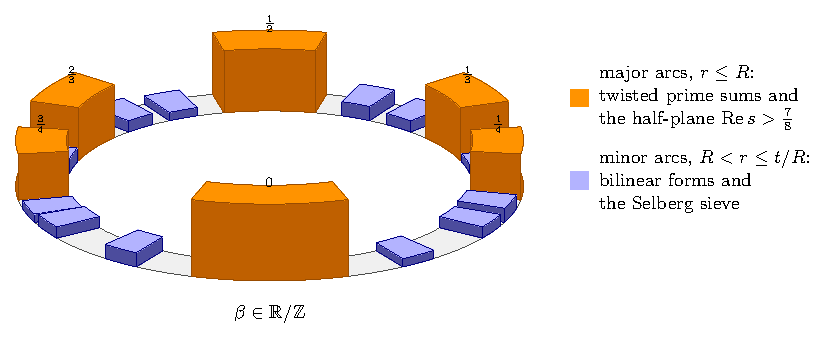
\includegraphics[width=\textwidth]{figures/fig_arcs.pdf}
\caption{The dissection of $\mathbb R/\mathbb Z$ in the proof of
Proposition~\ref{prop:hsum}, drawn for $R=4$. Near a fraction $a/r$ with $r\le R$ (major arcs)
the sum $A(t)$ is controlled by the twisted prime sums of Corollary~\ref{cor:prime}; elsewhere
(minor arcs) by Theorem~\ref{thm:mv}. The heights only indicate that the major arcs carry the
large values.}
\label{fig:arcs}
\end{figure}

\begin{proof}[Proof of Theorem~\ref{thm:pv}]
The character $\bar\chi$ is primitive modulo $q$. If $\log q\ge200$, then
Proposition~\ref{prop:hsum} for $\bar\chi$ and Lemma~\ref{lem:polya} give
\[
  \Bigl|\sum_{n\le x}\chi(n)\Bigr|\le\sqrt q\,(C_4\log\log q+6)\le(C_4+6)\sqrt q\log\log q.
\]
If $\log q<200$, then every sum $\sum_{m\le H}\bar\chi(m)e(m\beta)/m$ with $H\le q$ has modulus at
most $1+\log q<201$, and Lemma~\ref{lem:polya} gives
\[
  \Bigl|\sum_{n\le x}\chi(n)\Bigr|\le207\sqrt q\le\frac{207}{\log\log3}\sqrt q\log\log q.\qedhere
\]
\end{proof}

\section{The logarithmic derivative at \texorpdfstring{$s=1$}{s=1}}\label{sec:ek}

Recall that $\sigma_0=11/12+3/1000$ and that $K$ is the constant of Corollary~\ref{cor:prime}.

\begin{lemma}\label{lem:atone}
For every nonprincipal character $\chi$ modulo $q$,
\[
  -\frac{L'}{L}(1,\chi)=2\int_1^\infty\frac{S(\chi;t)}{t^2}\,dt,
\]
and the integral converges absolutely.
\end{lemma}

\begin{proof}
By Lemma~\ref{lem:mellin}(i) with $a=\chi\Lambda$, for real $s>1$,
\[
  \int_1^\infty S(\chi;t)\,t^{-s-1}\,dt=-\frac{L'}{L}(s,\chi)\,\frac1{s(s+1)}.
\]
As $s\to1^+$ the left side tends to $\int_1^\infty S(\chi;t)t^{-2}dt$ by dominated convergence,
since $|S(\chi;t)|\le Kt^{\sigma_0}\log(q+2)$ and $\sigma_0<1$. The function $L(s,\chi)$ is
entire and does not vanish at $s=1$ by Theorem~\ref{thm:zerofree}, so the right side tends to
$-\frac12\frac{L'}{L}(1,\chi)$.
\end{proof}

\begin{proof}[Proof of Theorem~\ref{thm:ek}(i)]
Let $\chi$ be nonprincipal modulo $q$, so $q\ge3$, and put
$Y=\bigl(\log(q+2)\bigr)^{1/(1-\sigma_0)}\ge1$. Since $|S(\chi;t)|\le\psi(t)\le4t$ by
Lemma~\ref{lem:chebyshev}(ii), Lemma~\ref{lem:atone} gives
\[
  \Bigl|\frac{L'}{L}(1,\chi)\Bigr|\le2\int_1^Y\frac{4\,dt}t
  +2K\log(q+2)\int_Y^\infty t^{\sigma_0-2}\,dt
  =\frac{8\log\log(q+2)+2K}{1-\sigma_0}.
\]
As $q+2\le q^2$, $\log\log(q+2)\le\log2+\log\log q$, and since $\log\log q\ge\log\log3>0$ the
right side is at most $C\log\log q$.
\end{proof}

For the lower bound in Theorem~\ref{thm:ek}(ii) we need to control the prime powers $n\le q^{25}$
with $n\equiv1\pmod q$. We count them in dyadic blocks with Selberg's sieve.

\begin{lemma}\label{lem:block}
Let $q$ be prime, let $M\ge1$ be an integer and let $1<z<q$. The number of $m$ with
$M\le m<2M$ for which $1+mq$ is a prime power is at most
\[
  \frac{2M}{\log z}+z(1+\log z)^2+z.
\]
\end{lemma}

\begin{proof}
If $1+mq=p^k$ with $p\le z$, then $p^k\in(Mq,2Mq)$, and for each prime $p$ at most one power of
$p$ lies in this interval, since $p^{k+1}\ge2p^k$. These $m$ number at most $z$. If $p>z$, then
$1+mq$ has no prime factor up to $z$, and we apply Lemma~\ref{lem:selberg} to the $M$ integers
$a_m=1+mq$, $M\le m<2M$, with $P$ the product of the primes up to $z$, $\nu(d)=1/d$ and $y=z$.
Every prime $p\le z$ differs from $q$, so for $d\mid P$ the condition $d\mid1+mq$ fixes $m$ in one
residue class modulo $d$, and $|R_d|\le1$. Here $g(l)=\prod_{p\mid l}(p-1)^{-1}$, which is the sum
of $1/n$ over the $n$ whose set of prime factors is that of $l$. Every $n\le\sqrt z$ has all its
prime factors at most $z$ and the product of its distinct prime factors is at most $\sqrt z$, so
\[
  S=\sum_{\substack{l\mid P\\l\le\sqrt z}}g(l)\ge\sum_{n\le\sqrt z}\frac1n\ge\frac{\log z}2.
\]
For squarefree $d$, $3^{\omega(d)}=\tau_3(d)$, and
$\sum_{d\le z}\tau_3(d)=\#\{(a,b,c):abc\le z\}\le z\bigl(\sum_{a\le z}1/a\bigr)^2\le z(1+\log z)^2$.
Lemma~\ref{lem:selberg} therefore bounds the number of these $m$ by $2M/\log z+z(1+\log z)^2$.
\end{proof}

\begin{lemma}\label{lem:progression}
There is an absolute constant $C_0$ such that for every prime $q\ge3$,
\[
  \sum_{\substack{1<n\le q^{25}\\n\equiv1\ (\mathrm{mod}\ q)}}\frac{\Lambda(n)}n
  \le C_0\,\frac{\log q\log\log q}q.
\]
\end{lemma}

\begin{proof}
Write $n=1+mq$ with $1\le m<q^{24}$, and let $J=\lfloor24\log_2q\rfloor+1$, so that $2^J>q^{24}$
and $J\le36\log q$. We split the range of $m$ into the blocks $2^j\le m<2^{j+1}$, $0\le j<J$
(Figure~\ref{fig:blocks}), and let $N_j$ be the number of $m$ in the $j$-th block with $1+mq$ a
prime power. We claim $N_j\le600\cdot2^j/(j+1)$. For $j<48$ this holds trivially. For $j\ge48$
apply Lemma~\ref{lem:block} with $M=2^j$ and $z=2^u$, $u=j/48\ge1$. Since
$2^j<2^J\le2q^{24}$, we have $z<2^{1/48}q^{1/2}<q$. Then $2M/\log z=96\cdot2^j/(j\log2)\le
150\cdot2^j/(j+1)$, and since $\log z\le u$,
\[
  z(1+\log z)^2+z\le2^u(2+u)^2\le\frac{441\cdot2^{4u}}{48u+1}\le\frac{441\cdot2^j}{j+1},
\]
because $(2+u)^2(48u+1)\le9u^2\cdot49u=441u^3$ and $u^3\le2^{3u}$. This proves the claim.

A term of the $j$-th block has $\Lambda(n)\le\log(1+2^{j+1}q)\le(j+2)\log2+\log q$ and
$n>2^jq$, so the block contributes at most
\[
  \frac{600}{(j+1)q}\bigl((j+2)\log2+\log q\bigr)\le\frac{600}q\Bigl(2\log2+\frac{\log q}{j+1}\Bigr).
\]
Summing over $j<J$ and using $\sum_{j<J}1/(j+1)\le1+\log J$, $J\le36\log q$ and
$\log J\le4+\log\log q$, the sum in the lemma is at most
$\frac{600}q\bigl(51\log q+5\log q+\log q\log\log q\bigr)$. Since $\log\log q\ge\log\log3>1/11$,
this is at most $C_0\log q\log\log q/q$ with $C_0=600\cdot617$.
\end{proof}

\begin{figure}[ht]
\centering
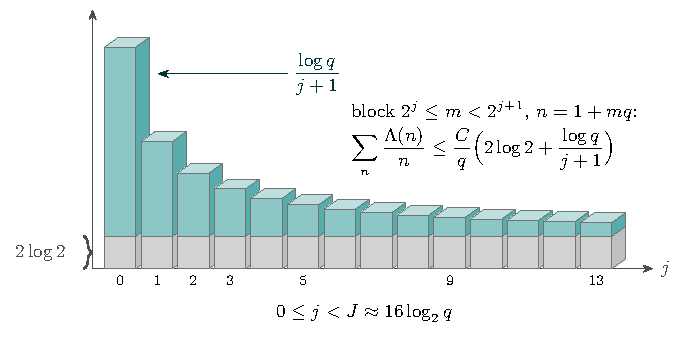
\includegraphics[width=0.85\textwidth]{figures/fig_blocks.pdf}
\caption{The dyadic blocks in the proof of Lemma~\ref{lem:progression}. The block
$2^j\le m<2^{j+1}$ contributes a constant part, of total size $\ll J\ll\log q$, and a part of
size $\log q/(j+1)$, whose total is $\ll\log q\log J$. The second part produces the factor
$\log\log q$.}
\label{fig:blocks}
\end{figure}

\begin{proof}[Proof of Theorem~\ref{thm:ek}(ii)]
Let $q\ge3$ be prime and put $c(n)=\sum_{\chi\ne\chi_0}\chi(n)$, the sum over the nonprincipal
characters modulo $q$. By orthogonality $c(n)=(q-1)\mathbf 1[n\equiv1\ (\mathrm{mod}\ q)]
-\mathbf 1[q\nmid n]$. Put
\[
  T(t)=\sum_{\chi\ne\chi_0}S(\chi;t)=\sum_{n\le t}c(n)\Lambda(n)\Bigl(1-\frac nt\Bigr),\qquad
  I=\int_1^\infty\frac{T(t)}{t^2}\,dt.
\]
By Lemma~\ref{lem:atone}, $\sum_{\chi\ne\chi_0}\frac{L'}{L}(1,\chi)=-2I$, so by~\eqref{eq:gammaq}
it suffices to show $-C\log q\le I\le C\log q\log\log q$.

By Corollary~\ref{cor:prime}(i), $|T(t)|\le qK\log(q+2)\,t^{\sigma_0}$. Let $Y=q^{25}$. Since
$25(\sigma_0-1)<-2$ and $\log(q+2)\le q$,
\[
  \Bigl|\int_Y^\infty\frac{T(t)}{t^2}\,dt\Bigr|\le\frac{qK\log(q+2)\,Y^{\sigma_0-1}}{1-\sigma_0}
  \le\frac{K\log(q+2)}{q(1-\sigma_0)}\le\frac K{1-\sigma_0}.
\]
For the lower bound, $c(n)\ge-1$ gives $-T(t)\le\psi(t)\le4t$, so
\[
  -I\le\int_1^Y\frac{4\,dt}t+\frac K{1-\sigma_0}=100\log q+\frac K{1-\sigma_0}.
\]
For the upper bound, $c(n)\le(q-1)\mathbf 1[n\equiv1\ (\mathrm{mod}\ q)]$ gives
\begin{align*}
  \int_1^Y\frac{T(t)}{t^2}\,dt&\le(q-1)\sum_{\substack{n\le Y\\n\equiv1\ (\mathrm{mod}\ q)}}
  \Lambda(n)\int_n^\infty\Bigl(1-\frac nt\Bigr)\frac{dt}{t^2}\\
  &=\frac{q-1}2\sum_{\substack{1<n\le q^{25}\\n\equiv1\ (\mathrm{mod}\ q)}}\frac{\Lambda(n)}n,
\end{align*}
which is at most $\frac{C_0}2\log q\log\log q$ by Lemma~\ref{lem:progression}. Hence
\[
  I\le\frac{C_0}2\log q\log\log q+\frac K{1-\sigma_0},
\]
and both bounds follow since $\log q>1$ and $\log\log q>1/11$.
\end{proof}

\appendix
\section{Transfer parameters for the eleven-twelfths half-plane}
\label{app:parameters}

The purpose of this appendix is to check the numerical consequences of
changing the zero-free boundary. The arithmetic here does not prove the
zero-free theorem. It checks that the subsequent deductions use only the
cited zero-free input. No claim of novelty is made for these
elementary parameter choices.

\subsection{The contour and unsmoothing margins}
Put
\[
 \theta=\frac{11}{12},\qquad \delta=\frac1{2000},\qquad
 a=\theta-2\delta,\qquad
 \sigma_0=a+8\delta=\frac{2759}{3000}.
\]
We have $1/2<a<1$, $0<\delta<1/1000$, and $a+2\delta=\theta$.
Thus the hypothesis of Proposition~\ref{prop:riesz} follows from the
cited nonvanishing statement. That proposition gives
$|S(\chi;x)|\le Kx^{\sigma_0}\log(q+2)$.

In Corollary~\ref{cor:prime} choose $h=x^{47/50}$. The two exponents
arising from unsmoothing satisfy
\[
 \frac{49}{50}-\left(1+\sigma_0-\frac{47}{50}\right)
 =\frac1{3000}>0,\qquad
 \frac{47}{50}+\frac1{100}=\frac{19}{20}<\frac{49}{50}.
\]
The first inequality controls the difference of two Riesz means divided
by $h$; the second absorbs the logarithm in the short-interval error.
The prime-power correction is smaller still, since
$1/2+1/100<49/50$. Consequently the proof gives a twisted prime-sum
bound with exponent $49/50$, with constants depending only on the fixed
choice of $\delta$.

\subsection{Major arcs}
Partial summation gives, for $M\ge1$,
\[
 \sum_{m\le M}m^{-49/50}
 \le1+\int_1^M u^{-49/50}\,du
 =50M^{1/50}-49\le50M^{1/50}.
\]
The proof of Lemma~\ref{lem:major} therefore gives its stated bound
with $Y^{1/50}$ in the denominator and $C_2=100C_3$.

Let $L=\log q\ge200$ and $M=\lceil L\rceil$, as in
Proposition~\ref{prop:hsum}. Set $R=M^{16}$ and $Y=M^{1800}$.
The elementary inequalities $L\le M\le2L$ and
$e^{L/16}\ge(L/16)^4/24>L+1$ show $2\le R<q$.
For the last strict inequality it suffices that
$L^3>48\cdot16^4$, which holds for $L\ge200$.

In the major-arc contribution, $\log(qR+2)\le18M$,
$2+2\pi R\le8M^{16}$ and $1+L\le2M$. Hence
\[
 k(1+L)
 \le\frac{288M^{34}}{1800M^{36}\log M}\le1.
\]
Here $1800/50=36$, leaving two powers of $M$ beyond the required
numerator exponent $34$. The minor-arc estimate is unchanged:
$\rho(1+L)\le2/M\le1$. Finally
$\log Y=1800\log M\le3600\log L$, so the two smooth-number terms
contribute at most $7200e^{11}\log L$. These are exactly the constants
used in Proposition~\ref{prop:hsum}.

The old choice $Y=M^{700}$ would give $Y^{1/50}=M^{14}$, which does
not establish the displayed major-arc bound. Changing the boundary
without changing this parameter would leave an actual gap.

\subsection{The cyclotomic tail and progression sieve}
For the tail in Theorem~\ref{thm:ek}(ii), choose $Y=q^{25}$. The exact
margin is
\[
 25(1-\sigma_0)-2=\frac1{120}>0.
\]
Thus $q\log(q+2)Y^{\sigma_0-1}\le\log(q+2)/q\le1$ for $q\ge3$.
The corresponding old margin, with $17$ in place of $25$, is negative;
the old tail estimate cannot simply be retained.

Now $n=1+mq\le q^{25}$ implies $m<q^{24}$. Put
$J=\lfloor24\log_2q\rfloor+1$. Since
$\log2>56/81$ and $\log q>1$, we have
\[
 J\le\left(\frac{24\cdot81}{56}+1\right)\log q<36\log q.
\]
The bound for $\log2$ follows from the first two terms of
\[\log2=2\sum_{j\ge0}\frac{(1/3)^{2j+1}}{2j+1}.\]

For $j\ge48$ use $u=j/48$ and $z=2^u$ in Lemma~\ref{lem:block}.
Then $1<z<2^{1/48}q^{1/2}<q$, and
\[
 \frac{2\cdot2^j}{\log z}
 =\frac{96\cdot2^j}{j\log2}
 \le\frac{150\cdot2^j}{j+1}.
\]
Indeed, $\log2>2/3$ and $(j+1)/j\le49/48$ make the ratio at most
$96(3/2)(49/48)=147<150$. For the remaining term,
\[
 (2+u)^2(48u+1)\le9u^2\cdot49u=441u^3\le441\,2^{3u}
 \quad(u\ge1),
\]
and therefore
\[
 2^u(2+u)^2\le\frac{441\cdot2^{4u}}{48u+1}
 \le\frac{441\cdot2^j}{j+1}.
\]
The elementary inequality $u\le2^u$ for $u\ge1$ follows, for example,
by minimizing $u\log2-\log u$. We obtain
$N_j\le591\cdot2^j/(j+1)\le600\cdot2^j/(j+1)$.
For $j<48$ the bound with $600$ is immediate from $N_j\le2^j$.

Summing the blocks as in Lemma~\ref{lem:progression} gives
\[
 \sum_{\substack{1<n\le q^{25}\\n\equiv1\pmod q}}
       \frac{\Lambda(n)}n
 \le\frac{600}{q}\bigl(56\log q+\log q\log\log q\bigr).
\]
Here $2(\log2)J\le72(\log2)\log q<51\log q$ and
$1+\log J\le5+\log\log q$. Since $\log\log3>1/11$,
the constant $C_0=600\cdot617$ suffices. The lower-bound integral
now contributes $4\log(q^{25})=100\log q$ in place of $68\log q$.
This completes the parameter verification used in the article.

\subsection{What was formally checked}
The three rational margin statements, including the two failures of the old
cutoffs, were proved using \texttt{norm\_num} in the accompanying
Lean file \path{ParameterAudit.lean}. Fresh axiom output lists only
\texttt{propext}, \texttt{Classical.choice} and \texttt{Quot.sound}.
The file does not claim to formalise all analytic estimates in this
appendix or to prove the cited zero-free theorem. The exact rational
Python program is a separate consistency check, with the same limits.

\section{Uniform transfer from a fixed zero-free boundary}
\label{app:uniformtransfer}

The role of the zero-free theorem can be separated from the numerical
choices of Appendix~\ref{app:parameters}. The following is a conditional
transfer statement; its proof supplies no independent zero-free theorem.

\begin{proposition}\label{prop:fixedboundary}
Fix $1/2\le\theta<1$. Suppose that every nonprincipal Dirichlet character
$\xi$ has $L(s,\xi)\ne0$ for $\Re s>\theta$. There exists $C_\theta>0$
such that every primitive character $\chi$ modulo $q\ge3$ satisfies
\[
 \sup_{x\ge0}\left|\sum_{n\le x}\chi(n)\right|
 \le C_\theta\sqrt q\log\log q.
\]
The constant is uniform in the modulus, the character and the summation
endpoint. Its dependence on $\theta$ is allowed.
\end{proposition}

\begin{proof}
Choose $\delta=\min(1/2000,(1-\theta)/100)$ and put
$a=\max(1/2,\theta-2\delta)$, $\sigma=a+8\delta$ and
$\eta=(1-\sigma)/4$. If $a=\theta-2\delta$, then
$\sigma=\theta+6\delta\le\theta+6(1-\theta)/100<1$.
If $a=1/2$, then $\sigma\le1/2+8/2000<1$.
Thus $1/2\le a\le1$, $0<\delta<1/1000$, $0<\eta\le1/8$ and
$a+2\delta\ge\theta$. Proposition~\ref{prop:riesz} therefore gives,
uniformly for nonprincipal $\xi$ modulo $k$,
\[
 |S(\xi;x)|\ll_\theta x^\sigma\log(k+2).
\]
The unsmoothing identity in Corollary~\ref{cor:prime}, with
$h=x^{(1+\sigma)/2}=x^{1-2\eta}$, gives
\[
 \left|\sum_{p\le x}\xi(p)\log p\right|
 \ll_\theta x^{1-\eta}\log(k+2).
\]
Here the difference of the two Riesz means divided by $h$ has exponent
$1-2\eta$, the interval error is $O(x^{1-2\eta}\log(2x))$, and the
prime-power error is $O(\sqrt x\log x)$. The inequality
$\log x\le x^\eta/\eta$ absorbs both logarithms; $\sigma\ge1/2$
ensures $1/2+\eta\le1-\eta$. Partial summation gives the corresponding
additively twisted prime bound.

The proof of Lemma~\ref{lem:major} now uses
\[
 \sum_{m\le M}m^{-1+\eta}\le M^\eta/\eta
\]
and gives the same conclusion with $Y^\eta$ in the denominator,
with an implied constant depending on $\theta$. For $L=\log q\ge200$
and $M=\lceil L\rceil$, take $R=M^{16}$ and $Y=M^A$, where $A$ is
an integer with $A\eta\ge36$ and $A\ge16$.
The minor-arc theorem is unchanged. Its weighted contribution is bounded
by $O(1+\log L)$, since $\rho(1+L)\le1$. For the major arcs the
coefficient after Abel summation is bounded by
\[
 \frac{R\log(qR+2)(2+2\pi R)(1+L)}{Y^\eta\log Y}
 \le \frac{288 M^{34-A\eta}}{A\log M}\le288.
\]
Finally, the two smooth-number contributions have total at most
$2e^{11}\log Y\le4Ae^{11}\log L$. This proves the harmonic-sum
bound $O_\theta(\log\log q)$ exactly as in
Proposition~\ref{prop:hsum}, including the case $Y\ge H$, in which
the nonsmooth sum is empty. Lemma~\ref{lem:polya} proves the result
for $L\ge200$. For $L<200$ its elementary harmonic bound gives
$207\sqrt q$, absorbed using $\log\log q\ge\log\log3>0$.
\end{proof}

This proposition proves the transfer from a fixed zero-free boundary to
the stated character-sum bound. It does not prove the existence of such a
boundary. Theorem~\ref{thm:zerofree} is the cited external result that supplies
that antecedent in the main application.

\section*{Source and computational material}
The source archive~\cite{BB26code} and the public preprint
\url{https://hexagonmath.org/2610.00256v2} provide the earlier coauthored
versions. Sources for this revision, vector figures, numerical checks and
separate verification notes are available in the same repository. The
parameter checks verify stated arithmetic margins; they do not establish
Theorem~\ref{thm:zerofree}.

\section*{Use of AI tools}
The earlier coauthored manuscript and Lean development used Claude under
the authors' direction, as recorded in the source archive. OpenAI Codex
prepared the explicit parameter conversion in Section~\ref{sec:riesz},
Lemma~\ref{lem:major}, Proposition~\ref{prop:hsum}, and the progression and
tail estimates in Section~\ref{sec:ek}. It expanded the Mellin inversion
justification and supplied Appendix~\ref{app:uniformtransfer}.
Appendix~\ref{app:parameters} identifies the exact numerical margins.
The authors remain responsible for the mathematics and references.

\begin{thebibliography}{99}

\bibitem{Bad10} A.~I. Badzyan, \emph{The Euler--Kronecker constant}, Math. Notes 87
(2010), 31--42. doi:\href{https://doi.org/10.1134/S0001434610010050}{10.1134/S0001434610010050}

\bibitem{BB26code} D.~Bhattacharjee and U.~Bhattacharya, \emph{The P\'olya--Vinogradov inequality
with $\log\log q$: Lean~4 formalisation and verification code}, GitHub release v1.2.0, 2026,
\url{\releaseURL}.

\bibitem{Dav00} H.~Davenport, \emph{Multiplicative Number Theory}, 3rd ed., revised by
H.~L. Montgomery, Grad. Texts in Math.~74, Springer, New York, 2000. doi:\href{https://doi.org/10.1007/978-1-4757-5927-3}{10.1007/978-1-4757-5927-3}

\bibitem{FLM14} K.~Ford, F.~Luca and P.~Moree, \emph{Values of the Euler $\phi$-function not
divisible by a given odd prime, and the distribution of Euler--Kronecker constants for cyclotomic
fields}, Math. Comp. 83 (2014), 1447--1476. doi:\href{https://doi.org/10.1090/S0025-5718-2013-02749-4}{10.1090/S0025-5718-2013-02749-4}

\bibitem{GS07} A.~Granville and K.~Soundararajan, \emph{Large character sums: pretentious
characters and the P\'olya--Vinogradov theorem}, J. Amer. Math. Soc. 20 (2007),
357--384. doi:\href{https://doi.org/10.1090/S0894-0347-06-00536-4}{10.1090/S0894-0347-06-00536-4}

\bibitem{HR74} H.~Halberstam and H.-E. Richert, \emph{Sieve Methods}, London Math. Soc.
Monographs~4, Academic Press, London, 1974.

\bibitem{Iha06} Y.~Ihara, \emph{On the Euler--Kronecker constants of global fields and primes
with small norms}, in: Algebraic Geometry and Number Theory, Progr. Math.~253, Birkh\"auser,
Boston, 2006, 407--451. doi:\href{https://doi.org/10.1007/978-0-8176-4532-8_5}{10.1007/978-0-8176-4532-8\_5}

\bibitem{IMS09} Y.~Ihara, V.~K. Murty and M.~Shimura, \emph{On the logarithmic derivatives of
Dirichlet $L$-functions at $s=1$}, Acta Arith. 137 (2009), 253--276. doi:\href{https://doi.org/10.4064/aa137-3-6}{10.4064/aa137-3-6}

\bibitem{MV77} H.~L. Montgomery and R.~C. Vaughan, \emph{Exponential sums with multiplicative
coefficients}, Invent. Math. 43 (1977), 69--82. doi:\href{https://doi.org/10.1007/BF01390204}{10.1007/BF01390204}

\bibitem{Mor18} P.~Moree, \emph{Irregular behaviour of class numbers and Euler--Kronecker
constants of cyclotomic fields: the log log log devil at play}, in: Irregularities in the
Distribution of Prime Numbers, Springer, Cham, 2018, 143--163. doi:\href{https://doi.org/10.1007/978-3-319-92777-0_8}{10.1007/978-3-319-92777-0\_8}

\bibitem{OAI26short} OpenAI, \emph{The Quasi-Riemann Hypothesis},
preprint (not refereed), 5 October 2026,
\href{https://github.com/openai/math/blob/1581d4cbdd69a0faf34b2089614fe2a814316a6a/preprints/The-Quasi-Riemann-Hypothesis-October-5-2026/paper2.pdf}{official repository copy}.
\bibitem{OAI26} OpenAI, \emph{The quasi-Riemann hypothesis: a zero-free half-plane
$\Re s>7/8$}, preprint (not refereed), 30 September 2026, with a Lean~4 formalisation, repository \url{https://github.com/openai/math}

\bibitem{Pal32} R.~E.~A.~C. Paley, \emph{A theorem on characters}, J. London Math. Soc.
s1-7 (1932), 28--32. doi:\href{https://doi.org/10.1112/jlms/s1-7.1.28}{10.1112/jlms/s1-7.1.28}

\bibitem{Was97} L.~C. Washington, \emph{Introduction to Cyclotomic Fields}, 2nd ed., Grad. Texts
in Math.~83, Springer, New York, 1997. doi:\href{https://doi.org/10.1007/978-1-4612-1934-7}{10.1007/978-1-4612-1934-7}

\end{thebibliography}

\end{document}
